\section{Appendix IV: The Estimate Tax Feature} \label{appendix4}


\begin{table}[ht!]
  \centering
  \begin{tabular}{|p{4cm}|p{12cm}|}
    \hline
    \textbf{Use Case}&\textbf{Description}\\
    \hline
    Estimate Tax&Based on the information entered and the current tax year,
                 calculate how much tax is due\\
    \hline
  \end{tabular}
  \caption{Calculate Tax Requirement}
\end{table}
\FloatBarrier

A feature to estimate tax would also be useful. Initially, this can be based on
the system used to calculate personal tax in the UK, where all of an
individual's income is added up and, depending on which threshold it reaches,
tax is deducted at that level. For example, for an individual earning
\pounds75,000 per annum from their job where he or she is a company employee,
initially their tax free allowance would be deducted from the gross figure,
then the basic rate is deducted from it up to its limit, then higher rate would
be deducted from the rest. However, if they have any income from sources which
have special taxation rules, such as interest on savings, these would be
deducted right after the personal allowance -- that is, income from special
taxation sources get added to the gross income figure, but tax from them is
deducted at a different rate and before the base tax. (\textsc{CITATION
NEEDED}).

There should be an option to allow a user to determine whether a transaction is
taxable. For income, the user should also be able to determine if it is already
net of tax (taxed at source) or if it's the gross amount, since this would
influence the tax calculation. Also, on expenditure, certain costs such as
memberships to professional organisations are deductible, so the user should be
able to indicate this when they are registering the category.

Furthermore, for the tax feature, it is important to emphasise that not all of
an individual's income will get taxed under income tax. For example, profits on
sales of shares gets taxed as capital gains tax. Since this type of tax is
outside of the scope of this application but would still appear on a user's
list of transactions, the system needs a way to highlight these so as for them
not to be included in the tax calculation.



Below is a wireframe to illustrate how the initial window for the
\emph{Estimate Tax} requirement\footnote{HM Revenue \& Customs (2018). Income Tax rates and allowances: current and past. Url: https://www.gov.uk/government/publications/rates-and-allowances-income-tax/income-tax-rates-and-allowances-current-and-past (visited on: 03 Mar. 2018).}:

\begin{figure}[ht!]
  \begin{center}
    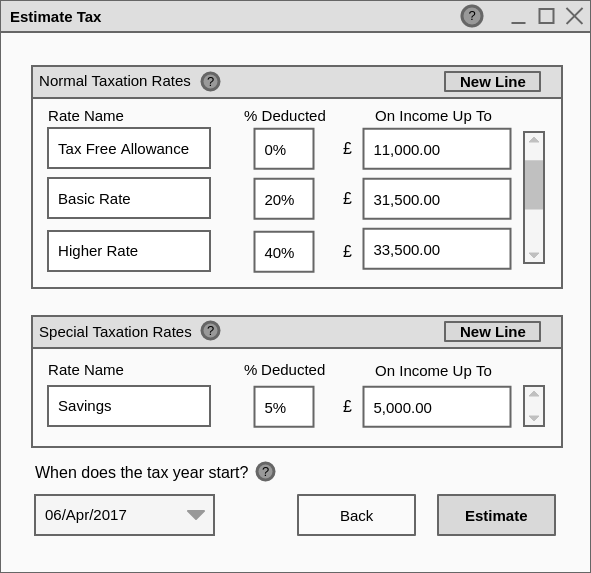
\includegraphics[width=14cm]{./contents/img/Wireframe_-_Estimate_Tax.png}
  \end{center}
  \caption{Estimate Tax interface. Date and allowances shown as specified by HM
    Revenue \& Customs }
  \label{fig:Wireframe.EstimateTax}
\end{figure}
\FloatBarrier

Normally, in the UK there is a difference between what is ``tax exempt'' and
what is ``taxed at 0\%''.  For the purposes of the estimation provided by
the requirements in this project, it was initially decided that this
distinction would be ignored, and that the user could simply have a choice to
use one of the dynamic boxes on \emph{Normal Taxation Rates} to indicate a tax
free allowance. However, due to the order in which the taxes are to be
deducted, it was decided that a non-taxable allowance field should still be
made available, but allow its value to be set to zero. This should allow for
more flexibility.

The interface would start with one line item, and then more items could be
added if the end user needs them. Each line represents one of the tax rates and
the threshold of income which needs to be reached before it starts deducting
tax at that percentage.

A choice has been made to include help texts next to the fields which are
likely to need them, and these are indicated in Figure
\ref{fig:Wireframe.EstimateTax} by the bubbles with the question marks next to
the relevant fields.



\subsection{Analysing the Estimate Tax Requirement}

This feature will allow the user to calculate an estimate of the amount of tax
due for a financial year, based on their income and expenditure. For this to
happen, the user will have to provide the date when the financial year begins,
and the tax tiers in their country. The tax estimation will be based as best as
possible on how personal tax is calculated in the UK \footnote{HM Revenue \& Customs, HM Treasury, Department for Work and Pensions, and Others . Personal tax: Income Tax. Url: https://www.gov.uk/topic/personal-tax/income-tax (visited on: 03 Mar. 2018).}. 

It was felt that Fowler's (\citeyear[][Session.~6.4-6.5]{fowler1997analysis})
\emph{Memo Account} and \emph{Posting Rules} patterns would be useful for this
case. Designing this requirement as such would ensure that, whenever the user
created a category which was deemed taxable, a portion of the income would be
posted to the tax account. It is also necessary to remember whether income has
already been deducted or if it relates to the gross amount, so this will have
to be taken into consideration. 


The \emph{Memo Account} pattern here will be implemented as tax-related
instances of \emph{Category}. Due to the double-entry principle of bookkeeping,
each tax instance will need to have a \emph{contra} category -- that is, a
second category which will act as the counterpart to the transaction -- so that
the principle is still observed.  In order for the user not to have to create
the transactions manually, however, an \emph{event listener} needs to be added
in order for entries to be made in the appropriate tax categories when
necessary. This is where the \emph{Posting Rules} pattern will be appropriate.
Below (Figure \ref{fig:ClassDiagram.Memo_Categories_and_Posting_Rule}) is an
analysis class diagram exemplifying the implementation:
\begin{figure}[ht!]
  \begin{center}
    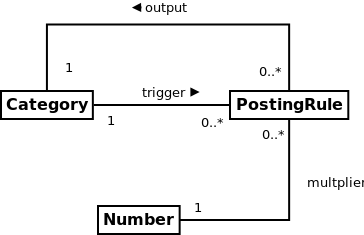
\includegraphics[width=9cm]{./contents/img/Class_Diagram_-_Memo_Categories_and_Posting_Rule.png}
  \end{center}
  \caption{}
  \label{fig:ClassDiagram.Memo_Categories_and_Posting_Rule}
\end{figure}
\FloatBarrier

So the principle being illustrated here is that, whenever an entry is posted to
a category which the user has marked as subscriber to tax, then the
\texttt{PostingRule}, which subscribes to that event, would determine whether a
transaction needs to happen between the tax category and its contra. Then, when
estimates need to be generated, they can simply come directly from the tax
categories.
